\documentclass[platex,a4j,10pt,twoside,twocolumn,dvipdfmx]{jsarticle}
\usepackage[ipaex]{pxchfon} % overleaf用
%

\setlength{\textheight}{240mm}

\setlength{\textwidth}{170mm}
\setlength{\oddsidemargin}{-15mm}
\setlength{\evensidemargin}{-15mm}
\addtolength{\textwidth}{15mm}

\setlength{\textwidth}{\paperwidth}
\setlength{\oddsidemargin}{-5.4truemm}  % 左の余白を20mm(=1inch-5.4mm)に
\setlength{\evensidemargin}{-5.4truemm} % 
\addtolength{\textwidth}{-40truemm}     % 右の余白も20mmに

\setlength{\topmargin}{-15mm}
\setlength\textfloatsep{3mm}
\setlength\floatsep{2mm}

\columnsep 1.0cm
%\setlength\abovecaptionskip{-3mm} %キャプションの前に挿入されるスペース

%------------------------------------------------------------



%------------------------------------------------------------
\usepackage[dvipdfmx]{graphicx}
% \usepackage{graphicx}
\usepackage{dendentitle}
\usepackage{mediabb}
\usepackage{url}
%\usepackage[dvipdfmx]{color}
\usepackage{color}
\usepackage{amsmath,amssymb,amsopn,bm}
\usepackage{subfig}
\usepackage{multirow}
\usepackage{cite}
\usepackage{comment}
%\usepackage{natbib}
\usepackage[table,xcdraw]{xcolor}

%------------------------------------------------------------ 関数定義
\renewcommand{\baselinestretch}{0.95}
\renewcommand{\figurename}{Fig.~}
\renewcommand{\tablename}{Table~}
\graphicspath{{./images/}}
\newcommand{\Tref}[1]{Table~\ref{#1}}
\newcommand{\Eref}[1]{式(\ref{#1})}
\newcommand{\Fref}[1]{Fig.~\ref{#1}}
\newcommand{\Sref}[1]{第\ref{#1}章}
\newcommand{\SSref}[1]{第\ref{#1}節}
\newcommand{\argmin}{\mathop{\rm arg~min}\limits}
\newcommand{\argmax}{\mathop{\rm arg~max}\limits}
\newcommand{\etal}[0]{\emph{et al}.~}

%タイトル
\title{Leveraging eBPF to Uncover the Characteristics of Shadow Attack}
\author{電子情報学専攻 修士課程2年 48-236427 手塚 尚哉}
\date{2024年5月10日}

\begin{document}
\makedendentitle{電子情報学中間報告資料}{落合研究室}
% TODO: Update the abstract with the final content. Note that this abstract is a placeholder 
% and should be updated with the final content.
% TODO: Update the abstract with the final content. Note that this abstract is a placeholder 
% and should be updated with the final content.

\section*{Abstract}
In the complex arena of cybersecurity, evasive malware,
such as shadow attacks that obscure malicious activities
through multiple processes, challenge conventional detection methods.
This paper introduces an innovative detection and analysis methodology
using Extended Berkeley Packet Filter (eBPF) technology to counteract these threats.
eBPF facilitates real-time, in-depth monitoring of system operations,
enabling the identification of sophisticated malware behaviors.

We leverage eBPF to trace process interactions and system calls,
identifying malicious patterns indicative of shadow attacks.
This approach distinguishes between legitimate and malicious activities
by analyzing process executions and network communications.
Despite challenges like data volume and behavior differentiation,
we apply smart filtering and machine learning to enhance detection accuracy.

Our research showcases eBPF's potential in detecting complex malware
through case studies, emphasizing the need for advanced analysis techniques
in cybersecurity.
This work contributes significantly to understanding and mitigating advanced malware threats,
proving eBPF as a vital tool in modern cybersecurity defenses.


\section{Introduction}
In the contemporary digital landscape, the sophistication of malware,
particularly in its ability to evade detection and analysis,
poses a significant challenge to cybersecurity efforts.
Among these evasive tactics, shadow attacks~\cite{Weiqin:ShadowAttack},
which cleverly distribute malicious activities across multiple processes,
stand out as particularly insidious.
These attacks exploit the inherent complexity of operating systems,
mimicking benign multi-process behavior to obfuscate their malicious intent.
Traditional detection mechanisms, reliant on static and dynamic analysis techniques,
often fall short in identifying these distributed threats,
necessitating the exploration of more advanced methodologies.

This paper introduces an innovative approach to tackling the
challenge posed by shadow attacks through the use of Extended Berkeley Packet Filter (eBPF).
eBPF, a technology that allows for the safe execution of custom code within the
Linux kernel without changing kernel source code or loading kernel modules,
offers a powerful mechanism for monitoring and tracing system-level operations.
Our research leverages eBPF to analyze the interconnections between function calls,
thereby revealing the execution patterns of processes involved in shadow attacks.
By mapping these patterns, we aim to uncover the stealthy operations of evasive malware,
providing insights that could lead to more effective detection and mitigation strategies.

We focus on the potential of eBPF to provide granular visibility into the behavior
of systems at runtime, enabling the identification of the complex orchestration of
processes characteristic of shadow attacks. Through the detailed analysis of function
call chains, we can trace the flow of execution within malicious processes,
identifying their strategies and mechanisms. This approach not only enhances
our understanding of how such attacks are constructed and executed but also opens
new avenues for developing countermeasures that can detect and neutralize these threats more efficiently.

By employing eBPF to dissect the intricacies of process execution and interaction in the
context of shadow attacks, we believe our research will contribute a novel perspective to the field of
cybersecurity. We demonstrate how eBPF's capabilities can be harnessed to advance our
understanding of malicious process execution, offering a promising methodology for combatting
evasive malware. Through this work, we aim to bolster the cybersecurity community's arsenal against
the ever-evolving landscape of malware threats, ensuring a more secure digital environment for all users.

Our exploration into the use of eBPF against shadow attacks not only highlights the adaptability and
complexity of modern malware but also underscores the necessity for innovative detection and analysis
techniques. As we delve into the capabilities and applications of eBPF, we pave the way for future
research and development in the domain of cybersecurity, seeking to establish more sophisticated defenses
against the cunning and elusive nature of malware attacks.


\section{Related Work}
\subsection{Malware Analysis}
Malware analysis is a critical aspect of cybersecurity, enabling the identification
and mitigation of malicious software threats.
Analysis techniques can be roughly categorized into two classes: static and dynamic.

\subsubsection{Static Analysis}
Static analysis involves examining the structure and content of a suspected malicious file without executing it.
Static analysis are often conducted as a preliminary step to grasp the general characteristics of the malware
before more sophisticated analysis techniques are applied \cite{chakkaravarthy2019survey}.

\textbf{Signature matching} is a common technique that compares the "signature", characteristics of a file
against a database of malware such as VirusTotal \cite{VirusTot28:online}. The characteristics include file size, hash values, and byte sequences.
Although this method has been a staple in malware detection, it is limited by its inability to detect only known malware.

\textbf{Disassemble and decompile} is another static analysis technique
that involves converting the binary code of a malware into a human-readable format.
From the decompiled code, analysts might be able to identify the malware's functionality and behavior as well as finding
interesting strings like URLs, IP addresses, and encryption keys.

\subsection{Dynamic Analysis \cite{10.1145/3329786}}
Dynamic analysis entails examining the behavior of malware by executing it in a controlled environment.
This approach enables analysts to witness the interactions between the malware and the system,
providing insights into its true intentions and capabilities.

\textbf{Function call analysis} is a method that focuses on tracking functions issued by the malware and the parameters
passed to them. One way to archive this is by code injection, in which analyzing code is hooked into
a specific function call and various information is collected and notified when the function is called.
Carsten et al. \cite{willems2007toward} created an automated malware analysis system that injects DLLs within CWSandbox,
letting analysts monitor system calls.

\textbf{Data flow tracking} is another approach that tracks the flow of data through the malware, and data tainting is an established
technique in this area. It involves marking (or "tainting") specific data components and then monitoring
how this tainted data propagates through the system.
Data tainting could be utilized in static analysis, but due to some evasion strategies like encryption and obfuscation
it has endured challenges in practice \cite{alashjee2019dynamic}.
SELECTIVETAINT \cite{chen2021selectivetaint} was invented to address performance overhead issue by employing static binary
rewriting to selectively instrument only instructions related to taint analysis.


\subsection{Shadow Attack \cite{Weiqin:ShadowAttack}}
Shadow Attack is one of the techniques used by malware writers to evade behavior-based detection systems,
orchestrating multiple processes to stealthily carry out malicious activities.

Such detectors typically rely on comparing system call graph within a process under scrutiny with predefined
malware specifications established on specific sequences or graphs of system calls\cite{inproceedings}.
For example, the malware specification of download-and-execute is expressed as follows \cite{Weiqin:ShadowAttack}:
\begin{equation}
  \texttt{recv} \land \texttt{open} \rightarrow \texttt{write} \rightarrow \texttt{exec}
\end{equation}
, where $s_1 \land s_2$ denotes both of two system calls $s_1, s_2$ are executed and $s_1 \rightarrow s_2$
denotes $s_1$ is followed by $s_2$.

So more specifically, the goal of Shadow Attack is to bypass dynamic malware detection based on
the analysis of system call graphs by exporting any critical system call included in malware specifications to
other collaborating processes, which is called shadow processes.
We call the Communication shadow processes do with each other as Shadow Process Communication (SPC).
The concept of Shadow Attack is illustrated in \Fref{img:shadow-attack}.
\begin{figure}[tp]
  \begin{center}
    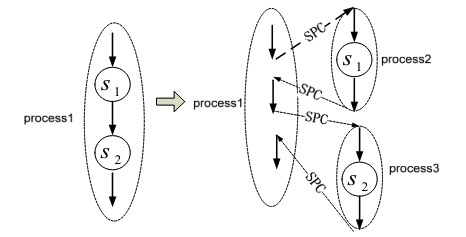
\includegraphics[width=\columnwidth]{./img/archi_SA.png}
  \end{center}
  \caption{Illustration of Shadow Attacks
    \cite{Weiqin:ShadowAttack}}
  \label{img:shadow-attack}
\end{figure}

Shadow attacks can be categorized into in-host, remote-network-coordinated, and hybrid.
In in-host shadow attacks, all shadow processes are executed on the same host and SPCs are conducted through
unix domain socket or stream pipe, while remote-network-coordinated shadow attacks involve multiple remote hosts
that are connected through network sockets.
Prototype implementation is made by the authors only for in-host shadow attacks.

One countermeasure is extracting correlation between processes and reconstructing
the original system call graph, but the authors conducted an evaluation experiment following this approach,
whose result suggested that solution would encounter challenges of high overhead.

\subsection{eBPF}
\subsubsection{Berkeley Packet Filter}
Steven and Van \cite{mccanne1993bsd} proposed the BSD Packet Filter architecture in 1993 for efficient packet capture on
Unix-based operating systems. In the following, we refer to Berkeley Packet Filter as "BPF."
At the time of paper publication, packet capture involved copying all packets acquired in the kernel
space to the user space before filtering.
This process resulted in unnecessary overhead. \cite{mccanne1993bsd} devised a pseudo-machine (BPF pseudo-machine)
that interprets programs written in special 32-bit instructions to perform filtering.
By running this pseudo-machine in the kernel space, they addressed the issue. Compared to existing systems,
BPF operated up to 20 times faster.
The overview of BPF architecture is shown in Figure \ref{img:bpf_old}.

BPF was introduced in the Linux kernel as "Linux Socket Filter" in version 2.1.75 and
was used to accelerate the \texttt{tcpdump} command.

\subsubsection{Extended Berkeley Packet Filter}
BPF underwent significant improvements and extensions in the Linux kernel version 3.18,
leading to the emergence of extended BPF, commonly referred to as eBPF \cite{Linux31836:online}.
The enhancements cover various aspects, with notable additions summarized below \cite{learning-ebpf}:
\begin{itemize}
  \item 64-Bit BPF Instruction Set: The BPF instruction set was reworked from 32-bit to 64-bit, resulting in improved execution efficiency.
  \item eBPF Maps: The introduction of eBPF maps allowed data sharing between user space and kernel space. These maps serve as a mechanism for efficient communication.
  \item eBPF Verifier: To ensure safe execution of eBPF programs, an eBPF verifier was added. It validates the correctness and security of eBPF code.
\end{itemize}

\begin{figure}[tp]
  \begin{center}
    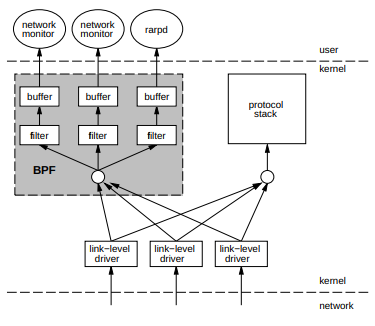
\includegraphics[width=\columnwidth]{./img/bpf_overview.png}
  \end{center}
  \caption{The overview of BPF architecture. It accelerates packet capture
    by performing filtering in the kernel space. \cite{mccanne1993bsd}}
  \label{img:bpf_old}
\end{figure}

The area covered by eBPF has also expanded.
In the context of networking, it has become able to handle various layers of the Linux network stack,
such as unix domain sockets and network devices.
Additionally, eBPF programs can now be used for performance tracing and enhancing the security of Linux systems,
leading to the term "BPF" losing its original meaning of "Berkeley Packet Filter" and being used as an independent term.

For convenience, BPF before the extension in v3.18 is sometimes referred to as classical BPF or cBPF.

\subsection{Overview of eBPF Architecture}
An overview of the eBPF architecture is shown in \Fref{img:ebpf-system}.
Hereafter, we describe the important processing flows with reference to \Fref{img:ebpf-system}.
\begin{figure}[tp]
  \begin{center}
    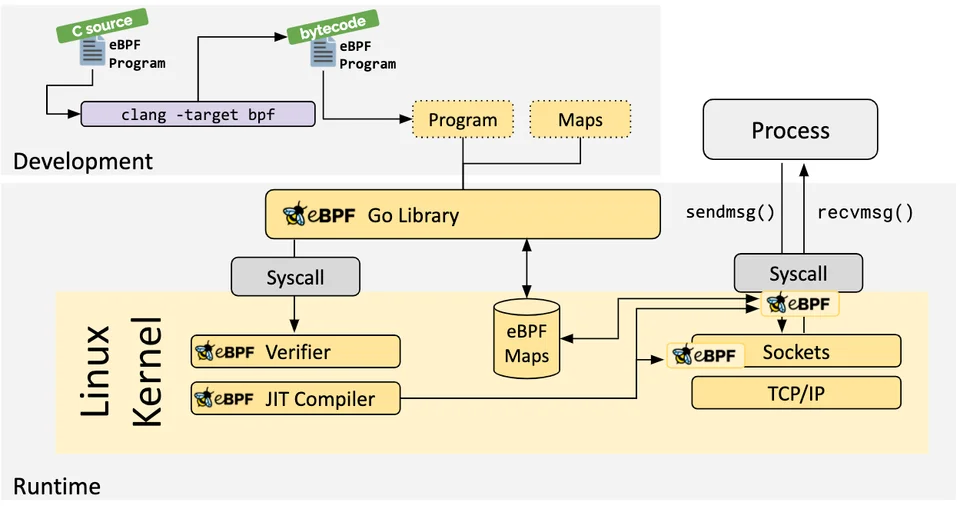
\includegraphics[width=\columnwidth]{./img/ebpf_system.png}
  \end{center}
  \caption{The overview of eBPF architecture. This figure shows how eBPF programs are compiled, verified, and executed.
    \cite{WhatiseB29:online}}
  \label{img:ebpf-system}
\end{figure}

\subsubsection{Event-Driven Architecture}

eBPF has an event-driven architecture.
The mechanism involves hooking an eBPF program to an event in the kernel, and then
performing the specified processing when the event occurs. eBPF programs can be dynamically loaded or removed.

The events that eBPF can hook into are defined as Program Types in the kernel's source code \footnote{\texttt{include/uapi/linux/bpf.h}}.
A few examples of Program Types are as follows:
\begin{itemize}
  \item XDP: An event for manipulating packets before data is copied to the kernel space when a packet arrives at a network device.
  \item Tracing: An event for detecting kernel function calls and passing tracepoints.
  \item LSM: An event for applying security policies using the Linux Security Module.
\end{itemize}
When such events occur, the eBPF program executes the processing corresponding to the Program Type.
For example, a program hooked to an XDP event can decide whether to accept or drop a packet.

\subsubsection{eBPF Verifier}
The eBPF verifier is a program that takes eBPF programs converted to bytecode as input and
verifies that they can be executed safely on the kernel.
The bytecode is loaded into the kernel via the \texttt{bpf()} system call
(shown as "Syscall" in \Fref{img:ebpf-system}), but the program will not run unless it passes verification by the verifier.
Specifically, it checks for things like avoiding memory access violations, ensuring the program exits normally,
and that the program is not granted unnecessary privileges.

In this way, the eBPF verifier enhances security by imposing restrictions on eBPF programs.
Since the verifier plays a crucial role in eBPF,
research has been conducted to mathematically verify the logic of the verifier \cite{vishwanathan2023verifying}.

\subsubsection{JIT Compilation}
The eBPF bytecode that passes the verifier is converted by a JIT compiler into machine code
that directly runs on the target CPU. This optimizes the execution speed, allowing it
to operate as efficiently as the kernel and kernel modules directly compiled from source code
\cite{WhatiseB29:online}.

\subsubsection{Kernel Modules}
Kernel modules are a mechanism that allows for the extension of kernel functions without modifying the kernel's
source code by loading object files during the execution of the Linux kernel.
Kernel modules are not subject to constraints like the eBPF verifier, thus offering a high degree of program freedom.
However, since kernel modules are executed with the same privileges as the kernel,
it is necessary to develop carefully to avoid embedding vulnerabilities \cite{chen2011linux}.

As Mayer et al. \cite{mayer2021performance} point out, avoiding the creation of kernel modules can be
considered an advantage of eBPF.


\section{関連分野}
\subsection{カーネルモジュール}
カーネルモジュールはLinuxカーネル実行時にオブジェクトファイルをロードすることで,
カーネルのソースコードを変更せずにカーネルの機能を拡張する仕組みの1つである.
カーネルモジュールには eBPF verifierのような制約がないため,プログラムの自由度は高い.
しかしカーネルモジュールはカーネルと同じprivilegeで実行されるので,
脆弱性を埋め込まないように注意して開発を行う必要がある \cite{chen2011linux}.

Mayerら \cite{mayer2021performance}が指摘するように,カーネルモジュールの作成を避けることができるのはeBPFの長所であると言える.

\subsection{Linux Security Modules}
LSM (Linux Security Modules) はLinuxカーネルのセキュリティポリシーを実装するためのフレームワークである.
LSMはアクセス制御に関するカーネル内の処理にフックポイントを提供し,そのポイントにセキュリティポリシーの
具体的な実装であるセキュリティモジュールを組み込むことができる
\footnote{セキュリティモジュールはカーネルモジュールのように動的にロードまたはアンロードすることができず,カーネルのビルド時に静的にリンクする必要がある.}.
カーネルがフックポイントを通過すると,セキュリティモジュールへのコールバックが発行されて強制的にアクセス制御が行われる.
LSMの処理フローの概要を\Fref{img:lsm-process}に示す.
\begin{figure}[tp]
  \begin{center}
    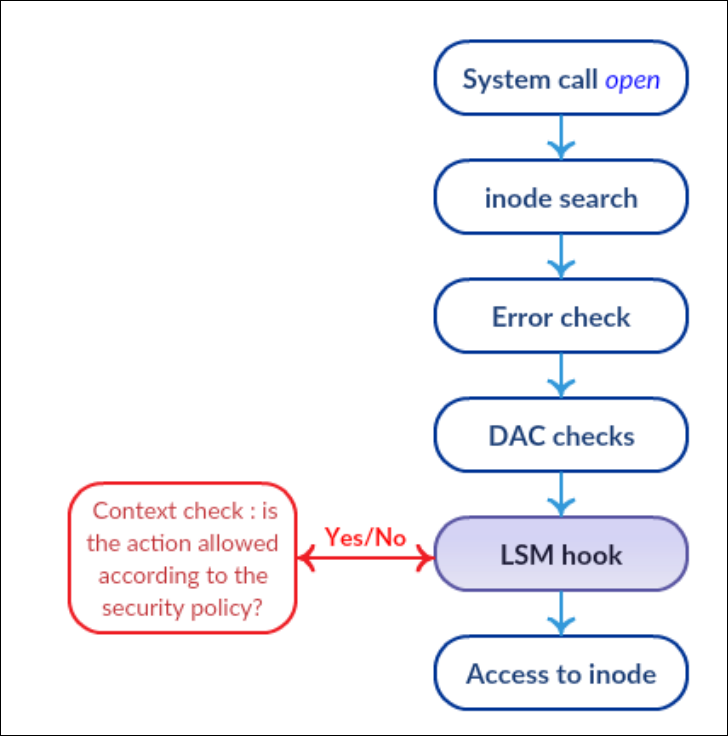
\includegraphics[width=\columnwidth]{./img/lsm-stack-hooks.png}
  \end{center}
  \caption{The process flow of LSM when \texttt{open()} system call is issued. \cite{LinuxSec12:online}}
  \label{img:lsm-process}
\end{figure}
LSMはLinuxのcapabilityやSELinuxで利用されている \cite{LinuxSec95:online}.

カーネルv5.17からLSM BPFという機能が追加され,eBPFプログラムをLSMが提供するAPIにフックすることができるようになった.

\subsection{Seccomp}
SeccompはLinuxで採用されているセキュリティシステムの1つで,あるプロセスが発行することができる
システムコールを制限する.
v6.6時点でSeccompの実装はcBPF (eBPFではない) に依存しており,cBPFを用いて
システムコールのフィルターをプロセスごとに変更することができる.
この機能をseccomp-bpfと呼ぶ.

SeccompはDocker \cite{Seccomps57:online} やKubernetes\cite{Configur55:online} などの仮想化技術で広く用いられている.

\subsection{クラウドネイティブ}
クラウドネイティブとは,クラウド基盤を前提としてアプリケーションやシステムを構築および管理するアプローチのことである.
物理インフラの調達とメンテナンスのコストが不要になるほか,アプリケーションの開発やデプロイが効率的になる点,
高い可用性が確保できる点がメリットとして挙げられる.

eBPFはクラウドネイティブ環境で幅広く使われている技術で,代表的なプロダクトとしてCilium \cite{CiliumCl38:online}がある.
Ciliumによってコンテナ間のL3通信を制御したり,セキュリティ機能や可観測性をコンテナ間パケットに付与したりすることができる.

eBPFは以下のような理由でクラウドネイティブ技術とよく適合する.
\begin{itemize}
  \item ネットワークやシステムコール,アプリケーションのイベントをリアルタイムで監視することができる.
  \item カーネル空間で実行されるためオーバーヘッドが小さく,スケーラビリティを損ねない.
  \item 動的なロードまたはアンロードが可能で,システムの継続的インテグレーション/デリバリーを容易にする.
\end{itemize}

\section{既存研究の取り組み}
これまでに述べたように,eBPFの応用範囲はパケットキャプチャにとどまらず
ネットワークスタック全般やシステムの監視にまで広がっている.
本章では,eBPFを活用したセキュリティシステムの中でも,ネットワーク領域の
事例とそれ以外の領域,そして両方に跨る事例をそれぞれ紹介する.

\subsection{DNSクエリのプライバシーの向上 \cite{rivera2020leveraging}}
この研究では,DNSクエリのプライバシーを毀損する攻撃についてまとめつつ,それらを緩和する方法の実現が
既存のシステムでは難しいことを主張している.そしてeBPFを利用して攻撃への対策を効率的に実施する手法を提案している.

\subsubsection{問題}
DoT (DNS over TLS)やDoH (DNS over HTTPS)といった暗号化プロトコルは,DNSクエリを暗号化することでネットワーク上の攻撃者が
クエリを盗聴することを防いでいる.しかしDoTやDoHで暗号化されるのはクライアントとキャッシュサーバの間の通信のみであり,
キャッシュサーバ上でクエリは復号化される.
したがってキャッシュサーバの運営者,典型的にはISP,はユーザとクエリ情報を結びつけることができるため,
クエリ情報からユーザのプロファイルを作成するde-anonymizationを試みる危険性がある.

RFC 7626はde-anonymizationへの対策の1つとして,アプリケーションごとにキャッシュサーバを変更することを
推奨している.これによりクエリの情報が分散するので,プロファイルの作成が難しくなる.

上記の対策を実施する方法は手動でDNSクライアントを設定する以外に存在せず,時間がかかる作業である上に実行効率も悪いという
問題点がある.

\subsubsection{提案手法}
この研究では,XDPでDNSまたはDoTのクエリパケットの宛先アドレスを編集することでクエリのリダイレクトを実行している.
提案手法によるDNSクエリの処理フローを\Fref{img:dns-process}に示す.
\begin{figure}[tp]
  \begin{center}
    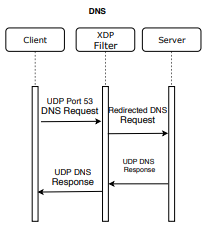
\includegraphics[width=45mm]{./img/dns-process.png}
  \end{center}
  \caption{DNS queries are intercept in XDP and eBPF implementation edits their destination. \cite{rivera2020leveraging}}
  \label{img:dns-process}
\end{figure}
XDPにフックされたeBPFプログラムはあるパケットがどのプロセスから送出されるかを認識しており,
key:プロセス名,value:宛先のハッシュマップを参照してクエリのアドレスを書き換える.
なお,この研究はDNSクエリを振り分けるキャッシュサーバのリストを指定できるuser-friendlyなインタフェースを提供している.

DoTではTLSで規定された処理を行う必要があるため,AF SocketというXDPの機能を使う.
先述したように宛先アドレスを編集したあと,AF Socketで作られた仮想ソケットにパケットを送信して
TCP handshakeやTLSの鍵交換を行う.

DoHにおいては,パケットがカーネルのネットワークスタックに到達する時点でクエリ情報は暗号化されているため,
平文のDNSやDoTと同様の方法を適用できない.そこでこの研究では,uProbes (user probes) にeBPFプログラムをフックして
DoHクエリの作成とレスポンスの復号化を監視した.
uProbesではデータがread-onlyであるためクエリの編集ができないが,その代わりに
クエリの情報があるキャッシュサーバにどの程度知られているかを計算し,閾値を超えたときにユーザに警告する実装を行った.

\subsubsection{評価}
Riveraらは\Fref{img:dns-net}に示す実験用ネットワークを構築して提案手法の評価を行った.
\begin{figure}[tp]
  \begin{center}
    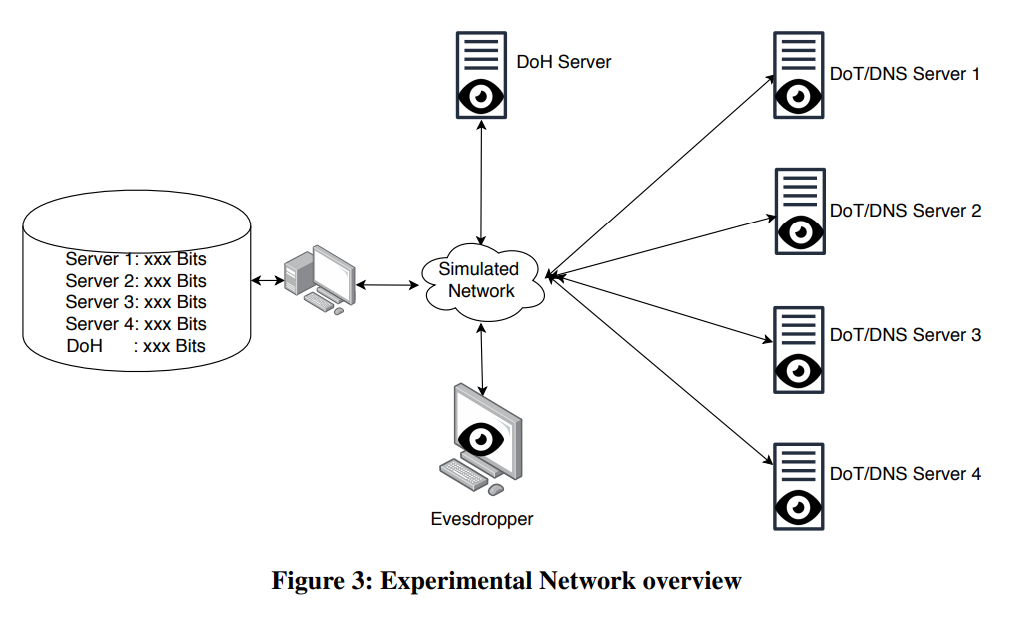
\includegraphics[width=\columnwidth]{./img/dns-eval-net.png}
  \end{center}
  \caption{The overview of the experimental network.}
  \label{img:dns-net}
\end{figure}

パフォーマンスの評価ではDNSとDoTにおける名前解決時間を計測した.その結果
DNSでは0.44\%,DoTでは8.15\%のオーバーヘッドが観測された.DoTでのオーバーヘッドが
大きいのは,AF Socketの処理がボトルネックになっている可能性がある.
DoHクエリの監視についてはCPUサイクル数を計測し,3.13\%のオーバーヘッドが見られた.

プライバシーの評価では,\Fref{img:dns-net}に示すキャッシュサーバ4台のそれぞれに
何ビットのクエリ情報が流出しているかを計算し,de-anonymizationが実行可能であるかどうかを
評価した.
DoT単体ではISPによるde-anonymizationが実行可能であったが,
DoTとeBPFを組み合わせた提案手法はクエリを異なるサーバにロードバランスすることで
de-anonymizationを防ぐことができることが示された.

\subsection{Programmabilityの高いシステムコールフィルタ \cite{jia2023programmable}}
本研究はLinuxのシステムコールのフィルタリング機構であるseccompの問題点を論じた.
そしてseccomp-bpfをeBPFに対応させることでフィルタに高いprogrammabilityを与え,
既存のseccomp-bpfよりも厳密なセキュリティポリシーを適用するためのデザインの提案と実装を行った.

\subsubsection{問題}
システムコールフィルタとは,システムコールのエントリーポイントにおいてそのシステムコールが
発行されることを許可または拒否するメカニズムのことを指す.
seccomp-bpfはプロセスごとに異なるフィルタをcBPFで記述して適用することができ,
カーネル空間で実行されるためパフォーマンスが優れている.

しかしcBPFがもつ以下の性質により,seccomp-bpfはプロセスごとに静的なallow listを
適用することしかできない.
\begin{itemize}
  \item ステートレスである
  \item プログラムサイズの上限が小さい (4096命令)
\end{itemize}
このため,本来許可するべきではないシステムコールを許可せざるを得なくなって
セキュリティが劣化したり,複雑なルールを複数のフィルタのチェインで表現しなければならないことで
実行効率が低下したりする.

seccomp-bpfの機能を補うためにseccomp notifier \cite{TheSecco46:online} が提案された.notifierは
システムコールが発行されるたびに実行コンテキストをユーザー空間からカーネル空間に移し,
そのシステムコールを許可または拒否する判断を行う仕組みである.
フィルタのprogrammabilityは高いものの,コンテキストスイッチに起因するオーバーヘッドが大きい.

\subsubsection{デザインと実装}
本研究では既存のseccomp-bpfをseccomp-cBPF,提案手法をseccomp-eBPFと呼び区別している.
seccomp-cBPFに欠落しているがシステムコールフィルタが有していると望ましい性質として,Jieらは4点を挙げていた.

1点目はstatefulnessである.statefulなフィルタはシステムコールの発行回数や頻度を記憶して
フィルタを運用することができる.また,プログラムの実行フェイズに応じて許可するシステムコールの集合を変化させる
precise temporal specializationも可能になる.

2点目はexpressivenessである.無駄のないフィルタを記述することでフィルタの効率が改善する.

3点目はsynchronizationである.システムコールの競合状態を利用する脆弱性が報告されており,
そのような脆弱性の原因となるシステムコールが並列に実行される場合に同期を取って競合状態を回避する.

4点目はsafe user memory accessである.システムコールの引数に
ポインタ型の変数が渡される場合,そのポインタが指す構造体を検査することはフィルタの意思決定において
有用である.例えば\texttt{open()}システムコールに渡されるポインタは開こうとしているファイル名の文字列を指している.

Jieらはこれら4つの性質を満たしつつ,
提案システムへの移行を容易にするためにのseccomp-cBPFが想定する脅威モデルを維持する実装を行った.
seccomp-eBPFの実装で特筆すべき点は以下の通り.
\begin{itemize}
  \item \texttt{BPF\_PROG\_TYPE\_SECCOMP}をProgram Typeに追加した.
  \item 既存のヘルパー関数を改修,あるいは新規の関数を追加した.
  \item 上記2点を検証するためにeBPF verifierの検証ロジックを変更した.
\end{itemize}

\subsubsection{評価}
seccomp-eBPFの機能の1つであるprecise temporal specializationの性能評価を行った.
実験では\Fref{img:tmp-spec}に示すようにサーバアプリケーションの実行フェーズを
初期化フェーズと機能フェーズに分け,それぞれのフェーズでのみ実行されるシステムコールの集合$S_{init}とS_{serv}$を
seccomp-eBPFのフィルタで許可した.これらのフィルタはプログラムの実行フェーズに応じて動的に適用された.
\begin{figure}[tp]
  \begin{center}
    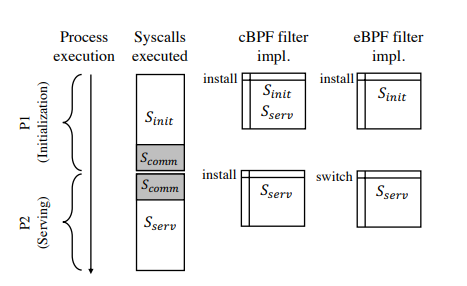
\includegraphics[width=\columnwidth]{./img/tmp-spec.png}
  \end{center}
  \caption{The concept of precise temporal specialization. It should be noted that
    the seccomp-cBPF filter in the initialization phase allows $S_{serv}$.}
  \label{img:tmp-spec}
\end{figure}
NGINXやMemcachedといったプログラムを用いて評価したところ,初期化フェーズにおいて33.6\%から55.4\%の
attack surfaceの削減が見られた.

さらに,precise temporal specialization以外に追加されたセキュリティ機能も評価された.
システムコールの実行回数を制限するcount limitingはCVE-2016-0728などの脆弱性をブロックし,
またserializationの機能はCVE-2018-18281を防ぐことに成功した.

パフォーマンスの評価では,\texttt{getpid()}システムコールを実行するマイクロベンチマークと,
サーバアプリケーションのベンチマークによるマクロベンチマークを扱った.

マイクロベンチマークの結果を\Fref{img:micro-bench}に示す.
\begin{figure}[tp]
  \begin{center}
    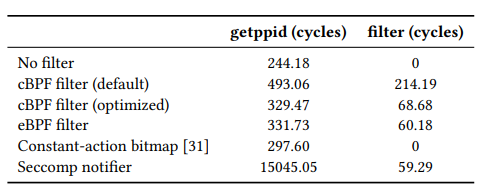
\includegraphics[width=\columnwidth]{./img/micro-bench.png}
  \end{center}
  \caption{Execution time of \texttt{getpid()} with different filters and filter execution time.}
  \label{img:micro-bench}
\end{figure}
seccomp-eBPFのフィルタは,seccomp-cBPFのフィルタよりもセキュリティが向上しているにも関わらず,
コンパイル時最適化を適用したseccomp-cBPFのフィルタと同程度のパフォーマンスを出した.
notifierのフィルタはシステムコール自体の実行時間を45倍程度大きくし,顕著な性能低下が見られた.

マクロベンチマークの結果を\Fref{img:macro-bench}に示す.図中の"hybrid"は
seccomp-cBPFとnotifierを組み合わせたフィルタである.
\begin{figure}[tp]
  \begin{center}
    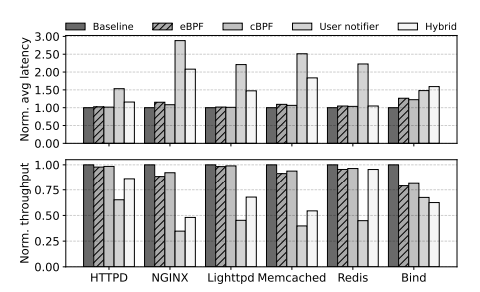
\includegraphics[width=\columnwidth]{./img/macro-bench.png}
  \end{center}
  \caption{Execution time of \texttt{getpid()} with different filters and filter execution time.}
  \label{img:macro-bench}
\end{figure}
同じ機能を実装したフィルタを適用した条件で,
\Fref{img:macro-bench}に示されるサーバアプリケーションを公式のベンチマークを用いて
レイテンシとスループットを評価した.
アプリケーションごとに差異は見られるが,マイクロベンチマークの結果と同様の傾向が見られた.

\subsection{周辺機器からLinuxを保護するフレームワーク\cite{tian2019lbm}}
本研究はBadUSBなどの悪意ある周辺機器を用いた攻撃や,周辺機器のプロトコルスタックのバグを突いた攻撃から
Linuxを保護するためのフレームワークを提案した.

\subsubsection{問題}
本研究が対象としている周辺機器はUSB,Bluetooth,NFCの3種類である.
周辺機器は各々のプロトコルに則ったパケットをカーネルとやり取りすることで動作するため,
attack surfaceとして悪意あるパケットを送信する方法と,カーネル側のプロトコルスタックの脆弱性を攻撃する
方法が考えられる.

しかしながら,USBを対象とした攻撃には系統的な対策が存在する \cite{tian2016making}が,
BluetoothやNFCには存在しない.
したがって,様々な周辺機器に対応することができる包括的なセキュリティフレームワークが必要である.

\subsubsection{デザインと実装}
この研究では,様々なプロトコルを扱うことができる拡張性の高いフレームワークとしてLBM,Linux (e)BPF Modules
を提案した.
そして,サポートする周辺機器のすべての入力と出力を検査すること,新しい周辺機器プロトコルの
サポートが容易であること,オーバーヘッドの小さいことなどを含むLBMが備えるべき7つの性質を整理した.

TianらはスタンドアローンなコンポーネントとしてLBMを実装した.
\Fref{img:kernel-design}にカーネル側のシステムの概要を示す.
\begin{figure}[tp]
  \begin{center}
    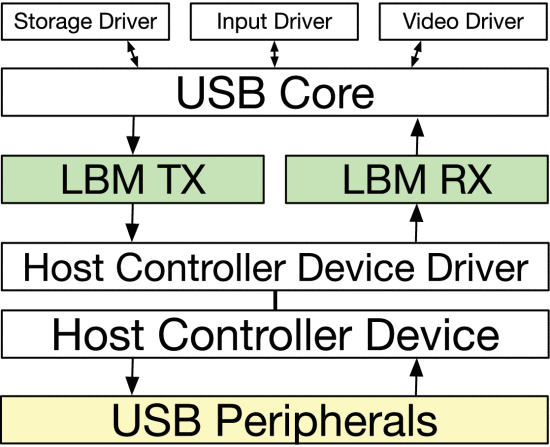
\includegraphics[width=\columnwidth]{./img/sodapdf-converted.png}
  \end{center}
  \caption{The overview of LBM in kernel side. \cite{tian2019lbm}}
  \label{img:kernel-design}
\end{figure}
eBPFでフィルタを適用するにあたって,eBPFプログラムのフックに2つのルールを定めている.
\begin{enumerate}
  \item eBPFプログラムをハードウェアのなるべく近くにフックする (フィルタが回避されることを防ぐため).
  \item 特定のハードウェアの実装に依存しない (拡張性を高めるため).
\end{enumerate}
このルールを満たすために,LBM TX (周辺機器への入力)とLBM RX (周辺機器からの出力) のフックポイントは
プロトコルスタックの下かつLinuxホストのコントローラーデバイスの上に配置された.

LBMを利用するユーザにはLBMTOOLというフロントエンドを提供した.
ユーザがPCAPに似たドメイン固有言語でフィルタのルールを記述すると,LBMTOOLはそれをコンパイルして
eBPFプログラムを生成し,フックポイントにロードする.

\subsubsection{評価}
LBMの評価にあたって,本研究では既知の攻撃を実施するケーススタディとベンチマークによるパフォーマンス計測を行った.

まずケーススタディでは,レスポンスパケットの先頭2バイトからパケット長をチェックすることで
スタックを保護するフィルタを記述することができた.
またUSB充電器を装ったBadUSBを充電は妨害せずにブロックできること,
Bluetoothの脆弱性の一つであるBlueBorne\cite{BlueBorn43:online}を10行程度のルールで対策できることを示した.
さらに概念実証としてLBMによるNFCのサポートを行った.その結果カーネルとLBMTOOLへのソースコードの変更は
合計で100行未満であり,拡張性の高さを表す根拠が得られた.

ベンチマークによるパフォーマンス計測では,マイクロベンチマークとマクロベンチマークが使用された.
マイクロベンチマークはRXパスで10,000のパケットをカウントし,LBMがもたらすオーバーヘッドを計測した.
その結果を\Fref{img:usb-latency}に示す.\Fref{img:usb-latency}によると,JITコンパイル
最適化が行われた場合LBMのオーバーヘッドは,パケットあたり1$\mu s$程度であった.
\begin{figure}[tp]
  \begin{center}
    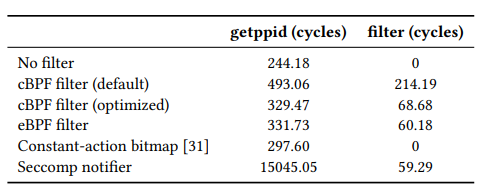
\includegraphics[width=\columnwidth]{./img/micro-bench.png}
  \end{center}
  \caption{LBM overhead in $\mu s$ measured on 10K packets on the RX path.
    For each subsystem, the 1st row is for normal LBM and the 2nd row is for LBM-JIT.\cite{tian2019lbm}}
  \label{img:usb-latency}
\end{figure}

マクロベンチマークでは,filebenchというベンチマークを採用してUSB3.0外部ストレージへのファイル書き込みのスループットを計測した.
その結果を\Fref{img:file-bench}に示す.VanillaはLBMが組み込まれていない純正のLinuxカーネルを意味している.
\begin{figure}[tp]
  \begin{center}
    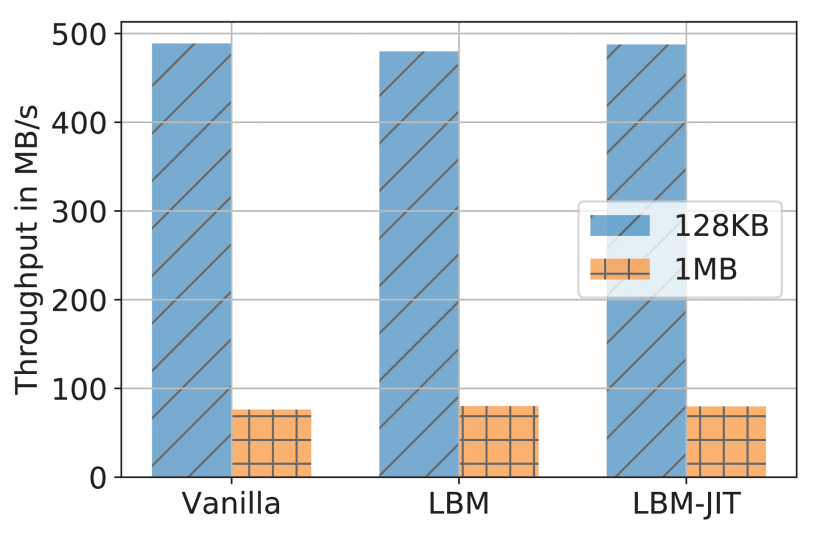
\includegraphics[width=\columnwidth]{./img/macro-graph.png}
  \end{center}
  \caption{Throughput of USB 3.0 external storage with filebench. \cite{tian2019lbm}}
  \label{img:file-bench}
\end{figure}
いずれの条件でも同様のスループットが得られており,LBMのオーバーヘッドが小さく抑えられていることを示している.
なお,平均ファイルサイズが大きくなるとスループットが極端に落ちる現象はページキャッシュサイズに由来する.

さらにBluetoothに対しても\texttt{l2ping}によるRTTの計測が行われた.\Fref{img:file-bench}の3種類の設定でRTTを計測したところ
いずれも5$ms$付近の結果が得られた.LBMによる1パケットあたりの遅延は1$\mu s$であったから,RTTと比較すると遅延は無視できる範囲に収まった.
% cloud nativeの話で0.5ページ, cloudflareで1ページ弱,abstractと「はじめに」で0.5ページ

\section{おわりに}
本稿では,eBPFという技術の発展の歴史,アーキテクチャ,主要なユースケースについて述べた後,
eBPFを活用したセキュリティシステムを提案する既存研究の取り組みを紹介した.
eBPFが提供するシステムの可観測性,セキュリティ,高パフォーマンスはセキュリティ技術者および研究者にとって
強力な武器であり,これまで以上に多岐にわたる問題に対処できるようになったことがわかる.

eBPFは比較的新しい技術であり,既に広く普及していながらも未だ発展途上である.
今後もクラウドネイティブ環境を中心に新規のユースケースが提案されることが期待される.

\bibliographystyle{unsrt}
{
  \footnotesize
  \bibliography{bib}
}

\end{document}
